\documentclass[tikz,border=8pt]{standalone}
% Shared look for every TikZ diagram. Load with \input{../../tools/tikz-style.tex}
\usepackage[T1]{fontenc}
\usepackage{lmodern}
\renewcommand{\sfdefault}{lmr}  % diagrams use the same serif as the text
\usetikzlibrary{arrows.meta, positioning, shapes.geometric, calc, fit, backgrounds}
\definecolor{cblue}{HTML}{4C78A8}
\definecolor{corange}{HTML}{F58518}
\definecolor{cgreen}{HTML}{54A24B}
\definecolor{cred}{HTML}{E45756}
\definecolor{cpurple}{HTML}{B279A2}
\definecolor{cgrey}{HTML}{6B6B6B}
\tikzset{
  every picture/.style={font=\sffamily, line width=1.2pt},
  box/.style={draw=#1, fill=#1!12, rounded corners=4pt, align=center, inner sep=7pt, minimum height=1.1cm},
  box/.default=cgrey,
  arrow/.style={-{Stealth[length=3mm]}, draw=cgrey, line width=1.4pt},
  title/.style={font=\sffamily\bfseries\Large},
  note/.style={font=\sffamily\small, text=cgrey, align=center},
}
\AtBeginDocument{\hyphenpenalty=10000 \exhyphenpenalty=10000}

\begin{document}
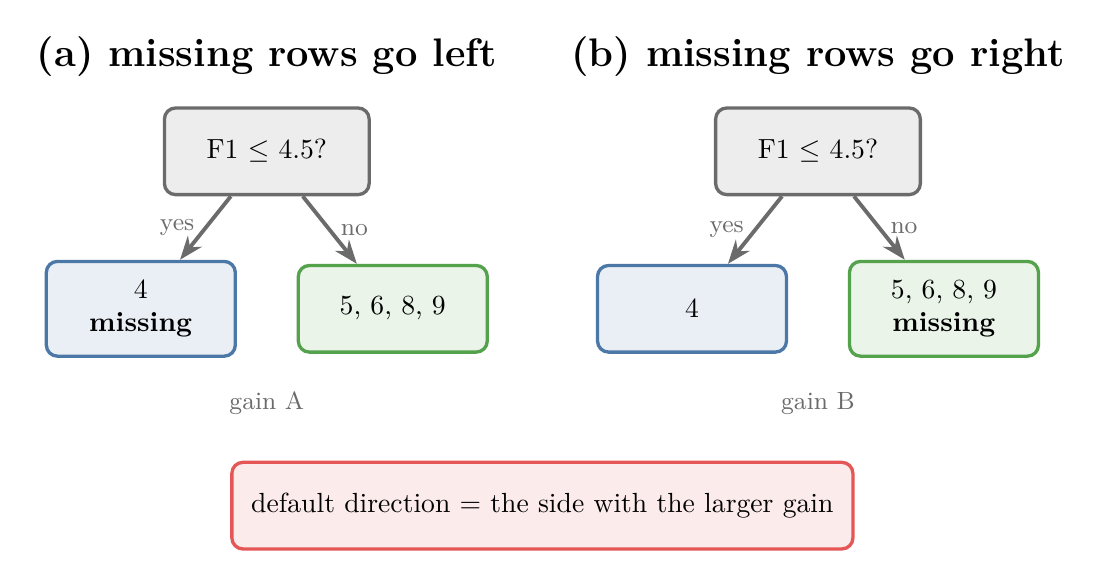
\begin{tikzpicture}[q/.style={box=cgrey, minimum width=2.6cm}, l/.style={box=cblue, minimum width=2.4cm},
  r/.style={box=cgreen, minimum width=2.4cm}]
  \node[title] at (0,1.6) {(a) missing rows go left};
  \node[q] (a) at (0,0.4) {F1 $\le$ 4.5?};
  \node[l] (al) at (-1.6,-1.6) {4\\\textbf{missing}};
  \node[r] (ar) at (1.6,-1.6) {5, 6, 8, 9};
  \draw[arrow] (a) -- node[note, left]{yes} (al); \draw[arrow] (a) -- node[note, right]{no} (ar);
  \node[note] at (0,-2.8) {gain A};
  \node[title] at (7,1.6) {(b) missing rows go right};
  \node[q] (b) at (7,0.4) {F1 $\le$ 4.5?};
  \node[l] (bl) at (5.4,-1.6) {4};
  \node[r] (br) at (8.6,-1.6) {5, 6, 8, 9\\\textbf{missing}};
  \draw[arrow] (b) -- node[note, left]{yes} (bl); \draw[arrow] (b) -- node[note, right]{no} (br);
  \node[note] at (7,-2.8) {gain B};
  \node[box=cred, minimum width=7cm] at (3.5,-4.1) {default direction = the side with the larger gain};
\end{tikzpicture}
\end{document}
